\documentclass[12pt, a4paper]{article}
\usepackage[utf8]{inputenc}
\usepackage{mdframed}
\usepackage{graphicx}
\pagenumbering{roman}
\usepackage{float}
% Title Page
\title{Development of a cyber security exercise}

\author{Kamil Glonek \\* Rafał Jaworowski \\* Aleksander Navitski}


\begin{document}
\graphicspath{ {images/} }
\maketitle
\pagebreak
\section*{Executive summary}
	\paragraph{}Cyber security is the body of technologies, processes and practices designed to protect networks, computers, programs and data from attack, damage or unauthorized access. Cyber security, also known as computer security or IT security includes controlling physical access to the hardware, as well as protecting against harm that may come via network access, data and code injection.
	
	\paragraph{}One of the most problematic elements of cyber security is the quickly and constantly evolving nature of security risks. Developers try to avoid such problems, but sometimes they just happens. Here we come with the help of finding the possible threats, risks and vulnerabilities that may have serious consequences. 
	
	\paragraph{}It is very important to teach especially young people how to handle with security gaps. The good practice is to practise a lot. We decided to prepare a set of exercises for the students. These tasks are to test web applications in order to improve it's security. We are sure that our research will deliver a lot of help in discovering IT security world.

\addcontentsline{toc}{section}{Executive Summary}
\pagebreak
\tableofcontents
\pagebreak
\pagenumbering{arabic}

\section{Introduction}
\subsection{Aim of this report}
\paragraph{}The main goal of this report is to familiarize what steps we have done concerning our research project. The report itself is only one part of our research. This paper summarize our findings in a pleasant way. Our hand in contains also different files. Final solution of our work is included in this report as well as in additional files.
\subsection{Team members}
\paragraph{} Our team consists of three people. All of us are IT Security students, taking part in Erasmus program. We are connected by the common goal, which is stated in the following part of the report. To achieve this goal, we are supervised this semester by FH-Prof. Mag. Dr. Simon Tjoa. Out tem members:

\paragraph{}
	\textbullet{} Kamil Glonek. Student of Information Technology at International Faculty of Engineering at Politechnika Łódzka (Poland). 
\paragraph{}
	\textbullet{} Rafał Jaworowski. Student of Information Technology at International Faculty of Engineering at Politechnika Łódzka (Poland). 
\paragraph{}
	\textbullet{} Aleksandr Navitski. Studying at Warsaw University of Technology, Faculty of Electronics and IT, Computer science branch (Poland).

\section{Problem statement}
\paragraph{} In this section our problem is desribed in detail, alongside with it's solutions considered. There is also considered our final approach.

\subsection{Project's topic description}
\textbf{Development of Cyber-security exercise / virtualized game environment}
\paragraph{}Cyber security exercises have been for a long time the ultimate learning experience for many students in some universities. Periodical competitions are organized between universities or inside one faculty where students play the role of attackers or defenders in a controlled and well defined environment.

\subsection{Problem recognition and possible solutions}
\paragraph{}Our topic could be analyzed at least in a few different ways. This led us to a brainstorming after which we decided to use some help of our supervisor concerning the final approach to the task.

\paragraph{}One of our ideas was to make a vulnerable application that will be installed in a earlier prepared Kali Linux system or other, with old version of apache2 server. This application would be written from scratch by us using few different technologies. It would of course improve our programming skills. But is really needed to help the future generations of students?Fortunately, with a help of our supervisor we realized that the better way would be to get use of already made training platforms.

\subsection{Final solution}
\paragraph{}After many hours of sitting and thinking about a perfect solution we all came up to one thing that may seem perfect. This solution is to make Lab exercises for students. These exercises will be about finding vulnerabilities in ready applications that will be mentioned in their tasks. The process of installation applications chosen by us will be fully automated. Student will be given a script file that will install everything for him. There will be also possibility of installing everything by the teacher using the same script file and easy tool called Ansible, for example.

\paragraph{}We think that this approach to the task is suitable for both, students and us. This way students will have more tasks to do, using fancy web applications. For us such a solution saves some programming and focuses more on preparing and finding tasks.

\paragraph{}The whole purpose of these exercises is purely educational, to ensure that students have an experiential training in IT security.

\section{Research project}
\subsection{Web applications}
\paragraph{}The process of research of finding Web applications, that would be from the one hand vulnerable and from the other hand not very obvious to hack, led us to choose following three web applications:\\*

\textbullet{} \textbf{OWASP WebGoat 2017} - deliberately insecure web application maintained by OWASP, designed to tech web application security. WebGoat trains developers not only how to exploit, but also how to fix and mitigate a vulnerablility.\\*

\textbullet{} \textbf{Google - Gruyere} - small, cheesy web application that allows customer to publish snippets of texts and also upload images. There is a bunch of stuff to learn - XSS, CSRF, Request hacking. The whole application is created using python and it does not use external database (no sql injection).\\*

\textbullet{} \textbf{BWAPP} - buggy web application with over 100 vulnerabilities.\\

\subsection{Tools}
\paragraph{}We reccomend to use Mozilla Firefox web browser for exploring these applications, but in case of not working XSS change the browser for example for Iceweasel. In order to make your life a little bit easier it is good for You to use also following tools that will help You with creating and modifying requests:\\

\textbullet{} \textbf{Ansible} - is a open-source automation engine that automates software provisioning, configuration management and application deployment. Ansible's main goals are simplicity and ease-of-use. It also has a strong focus on securitty and reliability, featuring a minimum of moving parts, usage of OpenSSH fo transport. Ansible helps us to manage multiple different machines at the same time wia SSH.\\

\textbullet{} \textbf{BurpSuite} - graphical tool for testing Web application security. Its various tools work seamlessly togethr to support the entire testing process from initial mapping and analysis of an application's surface, through to finding and exploiting security vulnerabilities. You may use this tool in order to eg. intercept proxy.\\*

\textbullet{} \textbf{WebScarab} - it is similar tool to BurpSuite. It serves as a proxy that intercepts and allows people to alert web browser web requests (both for HTTP and HTTPS) and web server replies.\\*

\textbullet{} \textbf{Nikto Web Scanner} - is a Web server scanner that tests servers for dangerous files/CGIs, outdated server software and other problems. It performs generic and server type specific checks. It also captures and prints cookies received.\\*

\textbullet{} \textbf{Vega Vulenarbility Scanner} - includes an automated scanner for quick tests and intercepting proxy for tactical inscpection. The Vega scanner finds XSS (cross-site-scripting), SQL injection and other vulnerabilities. \\*

\textbullet{} \textbf{Firefox Web Developer} - is an extension for Mozilla-based web browsers that adds editing and debuging tolls for web developers.\\*

\subsection{Used systems}
\paragraph{}For our purposes we used few different distributions of Linux operating systems. All these machines were running on VMware workstation running on Windows.\\
We used Kali Linux to run all chosen applications and tools. Kali Linux is good system for hacking as it has lot of pre-installed hacking tools. We used also Ubuntu system and we installed Ansible tool on it.

\subsection{Application installation}
In this section You will get to know how to install step by step every of previously mentioned applications.
\subsubsection{Installation of WebGoat 2017}
In order to install WebGoat web application one have to perform following steps on your Linux system:\\
\\
open terminal\\
Install java (if is not installed) with command:\\
sudo apt-get install default-jre\\
\\
Check version (should be $\rangle$ 1.6) using: \\
java -version\\
\\
Download WebGoat with wget:\\
https://s3.amazonaws.com/webgoat-war/webgoat-container-7.0-SNAPSHOT-war-exec.jar\\
\\
Now You can run webgoat with:\\
java -jar webgoat-container-7.0-SNAPSHOT-war-exec.jar\\
\\
Once it is running in your terminal go to any web browser and reach WebGoat typing in url adddress:\\
localhost:8080/WebGoat\\
\\
The main page of new WebGoat looks following:\\
\begin{figure}[H]
	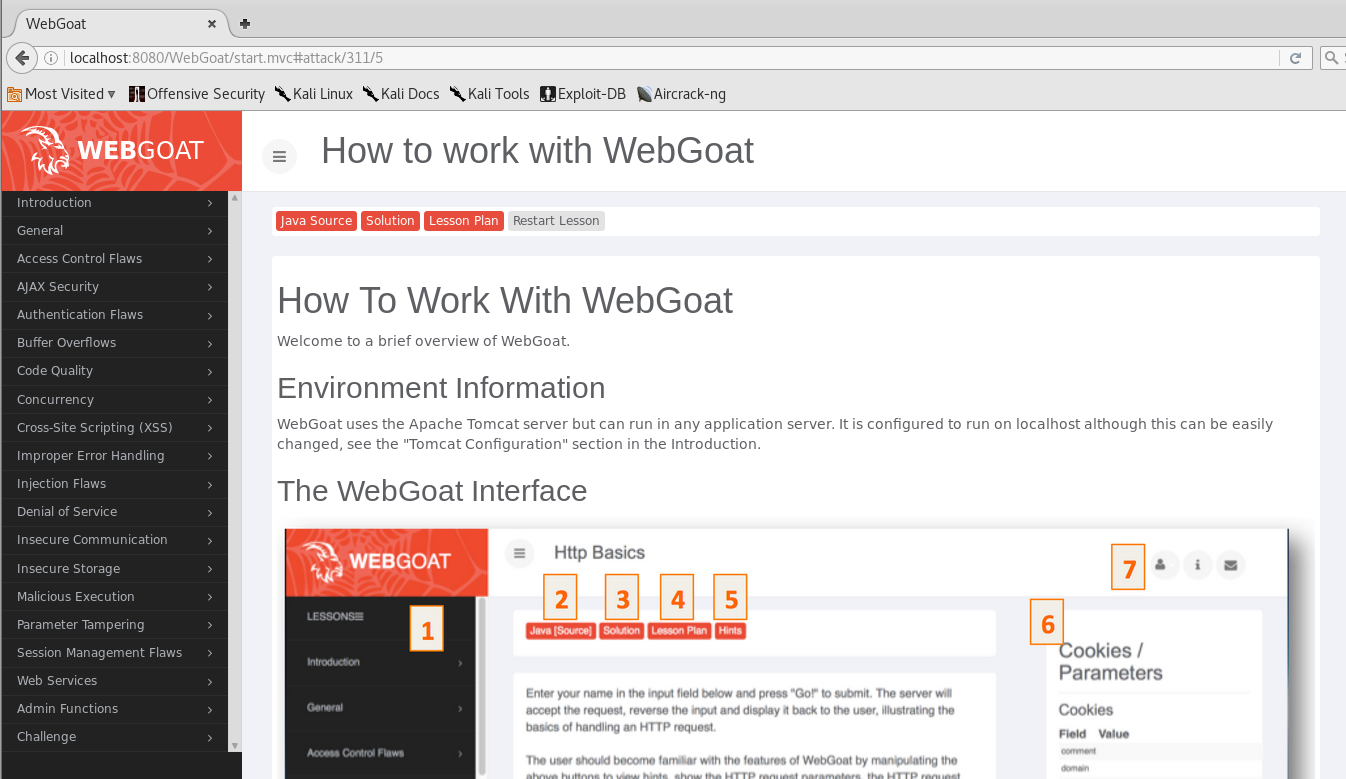
\includegraphics[width=1.0\textwidth]{webGoatStartPage.png}
	\caption{Start Page of WebGoat 2017}
\end{figure}

\subsubsection{Installation of Google Gruyere}
If you want manually install Google Gruyere type following commands:\\
\\
Create new directory for your application:\\
mkdir gruyere\_server\\
\\
Go to this newly created directory:\\
cd gruyere\_server\\
\\
Download application:\\
wget http://google-gruyere.appspot.com/gruyere-code.zip\\
\\
Unpack downloaded file in the same folder:\\
unzip gruyere-code.zip -d\\
\\
Now, run python application typing:\\
python gruyere.py\\
\\
Following application output instructions from terminal, in your browser go to:\\
127.0.0.1:8008\\
\\
The main page of Google Gruyere is depicted below:\\
\begin{figure}[H]
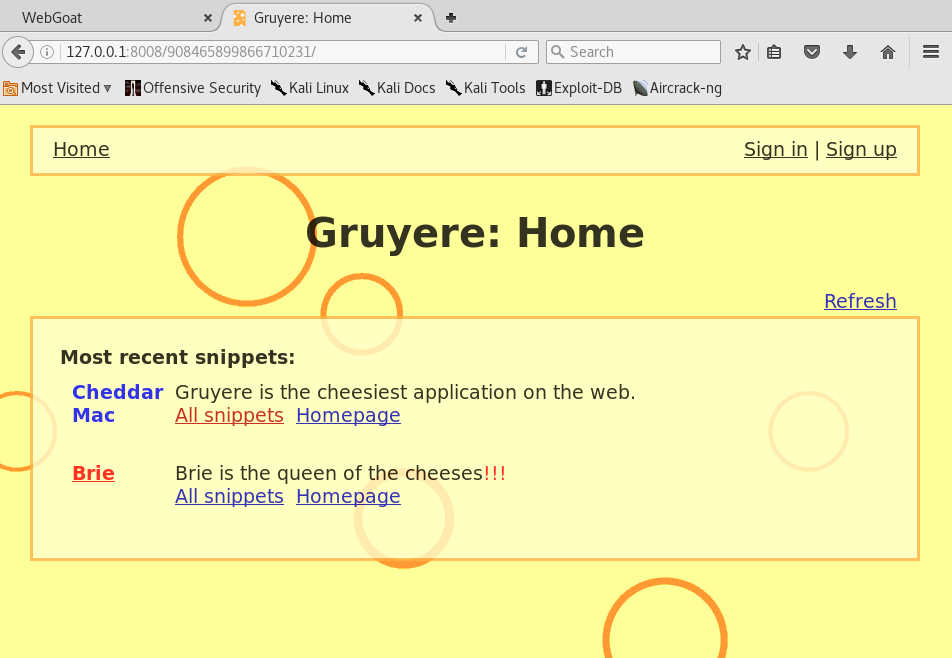
\includegraphics[width=1.0\textwidth]{googleGruyereStartPage.png}
\caption{Start Page of Google Gruyere}
\end{figure}

\subsubsection{Installation of BWAPP}
You may run BWAPP application with following:\\
\\
Download OWASP vulneable web apps and run it alongside your system in VMWare or in your local area network.\\
\\
in Your we browser go to:\\
192.168.30.135\\
\\
BWAPP's main page is presented at the following screenshot:\\
\\
\begin{figure}[H]
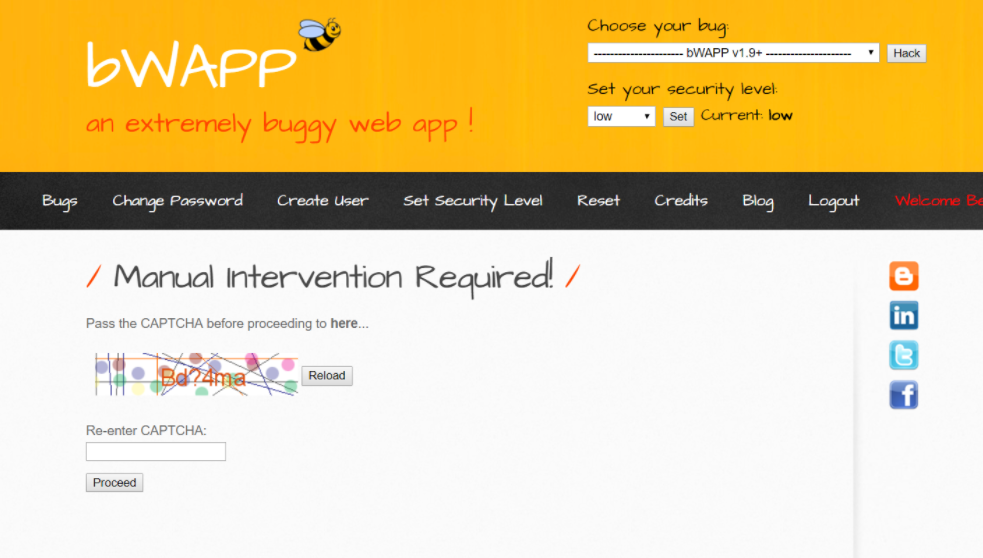
\includegraphics[width=1.0\textwidth]{bwappStartPage.png}
\caption{Start Page of BWAPP}
\end{figure}

\subsubsection{Installation of Ansible}
Machine on which we want install software must have ssh server enabled. Here are steps how to to accomplish that:\\
\\
apt-get install openssh-client\\
apt-get install openssh-server\\
service ssh start\\
\\
edit /etc/ssh/sshd\_config\\
PermitRootLogin yes\\
service ssh restart\\
\\
Below there is described a way of installing Ansible tool:\\
\\
sudo apt-add-repository ppa:ansible/ansible -y\\
sudo apt-get update\\
sudo apt-get install ansible -y\\
\\
ssh-keygen -t rsa -b 4096 -C “user@ubuntu”\\
ssh-copy-id ip\_address\\
eval `ssh-agent -s`\\
or\\
eval \$(ssh-agent)\\
ssh-add \~{}/.ssh/id\_rsa\\
\\
Now we are able to connect via ssh without password.\\
\\
Edit /etc/ansible/hosts\\
(web)\\
192.168.30.145 ansible\_ssh\_user=user\\
\\
ansible all -m ping\\
(should be success)\\
\\




\subsection{Automation of installation}
\paragraph{}Our task is also to make installation of all needed tools and applications really easy. That is why we prepared fully automated way to install it all in only few seconds on even multiple devices. We use Ansible tool which is very helpful in such a situations. The installation of this tool is described in the previous chapter. Together with the project we deliver ready script that will allow the teacher to install remotely, all desired applications on devices for it's students. The Ansible tool itself is very simple in usage. One has only to specify ip addresses of all computers in the network in '/etc/ansible/hosts' file. Next step is to create 'playbook.yml' file with the commands that he wants to perform on all hosts. In this file there are instructions on how to install scripts.\\

\paragraph{}In order ro run our three web applications when installed in automated way You have to run:\\
\\
For WebGoat 2017 type in your browser:\\
localhost:8080/WebGoat\\
\\
For Google Gruyere run in terminal (by default in root directory):\\
python gruyere.py\\
\\
For BWAPP go to:\\
localhost/bWAPP/install.php\\

\begin{figure}[H]
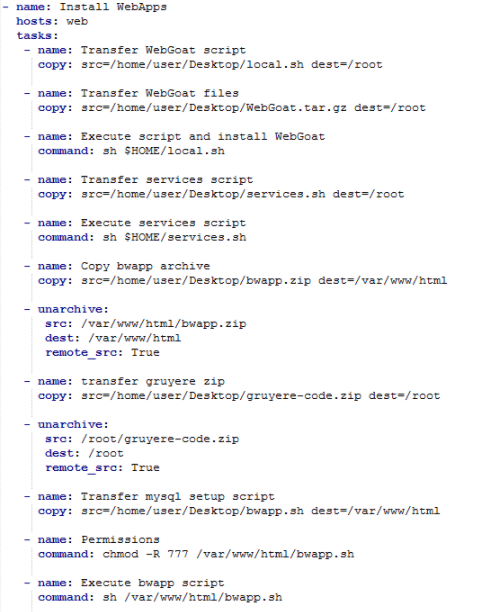
\includegraphics[width=1.0\textwidth]{playbook.png}
\caption{Example of playbook.yml file.}
\end{figure}

\begin{figure}[H]
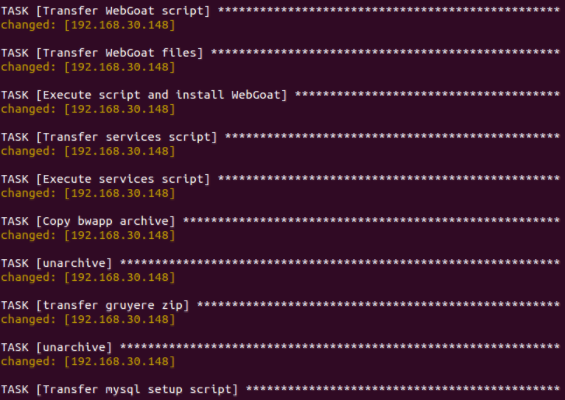
\includegraphics[width=1.0\textwidth]{playbookOutput.png}
\caption{Output of Ansible after execution of our playbook}
\end{figure}

\subsection{Automation scripts}
\paragraph{}For needs of our project and needs of teacher, in order to make his work easier we wrote same bash scripts. They are to install web applications automatically. The screenshots of one of these scripts are shown below. It is script with instruction on how to install WebGoat. All scripts are delivered in a package with final hand in.

\begin{figure}[H]
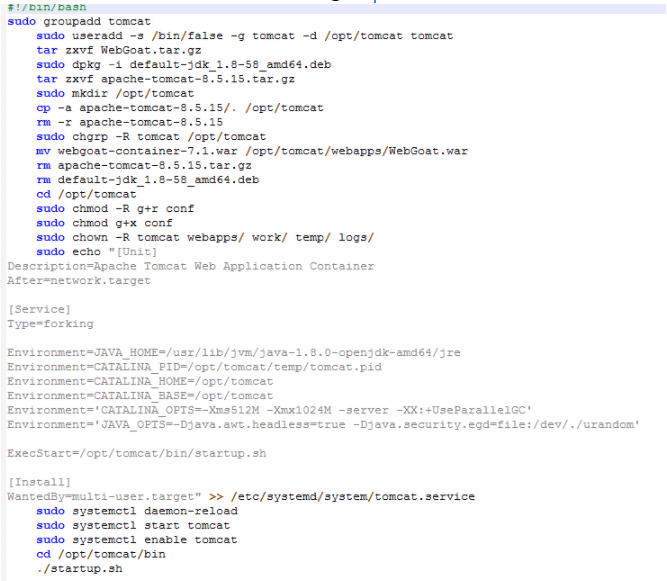
\includegraphics[width=1.0\textwidth]{webGoatScript.png}
\caption{WebGoat installation script}
\end{figure}

\newpage{}

\subsection{Exercise instructions}

\subsubsection{WebGoat exercise}
%\fbox{\begin{minipage}{33em}
		\begin{center} \textsc{WebGoat Exercise}
		\end{center}

WebGoat is really good vulnerable web application to start with, because it contains lots of hints for beginners.\\

1. Injection Flaws. Simple SQL injections.\\
\\
Injection flaws allow attackers to relay malicious code through an application to another system. These attacks include calls to the operating system via system calls, the use of external programs via shell commands, as well as calls to backend databases via SQL (i.e., SQL injection). Whole scripts written in Perl, Python, and other languages can be injected into poorly designed applications and executed. Any time an application uses an interpreter of any type there is a danger of introducing an injection vulnerability.\\
\\
a) In a Stage 1 tab: String SQL Injection try to login as an admin. (hint: Try to get use of Firefox Web Developer).\\
\\
b) In String SQL section display all card numbers of all users.\\
\\
c) Blind Numeric SQL Injection. Find the pin in the pins table for the cc\_number 1111222233334444 (SQLmap can be useful).\\
\\
d) Log Spoofing. Login as an admin in this section. Check the login for also for possibility of XSS.\\
\\
e) Can you find all users	that its name starts with letter ‘J’.\\
\\
2. Cross Site Scripting (XSS) attacks.\\
\\
Cross Site Scripting involves scripts being run by sites that reflect user input back to the browser‘s window without any context-sensitive output encoding. This results in code actually being executed instead of text being displayed.\\
\\
a) Phising with XSS\\
\\
Using XSS and HTML insertion.\\
i) Insert XSS and HTML credentials.
ii) Add javascript to actually collect the credentials.\\
\\
b) XSS attacks\\
i) Check if the website is vulnerable for XSS attacks. Input script that will show an alert message. Present what does the output look like in your case.\\
\\
ii) List 10 different payloads that works on this site.\\
\\
iii) Name few ways that the developer/programmer can avoid such a vulnerability.\\
\\
iv) Steal the cookie of the session. Describe briefly the way You did it. Send the cookie to some .txt file.\\
\\
d) Cross Site Request Forgery (CSRF)\\
\\
Describe how does CSRF work on a theoretical level. Present it in a form of a diagram and then:
Send the email to a newsgroup. The email contains malicious code hidden in a image whose URL is pointing to dangerous request. In this type of attack your message will be stored so anyone will can access the message. Remember to set the title interesting to gather more victims.\\
\\
3. XML injection\\
\\
XML Injection is an attack technique used to manipulate or compromise the logic of an XML application or service. The injection of unintended XML content and/or structures into an XML message can alter the intend logic of the application. Further, XML injection can cause the insertion of malicious content into the resulting message/document.\\
\\
Go to AJAX Security -$\rangle$ XML Injection\\
\\
Try to add more rewards to your allowed set of rewards by altering the response. Follow the hints on the website.\\
\\
4. Directory Traversal Attack\\
\\
A directory traversal attack is an exploit which allows attackers to access restricted directories and execute commands outside of the web server's root directory.\\
\\
Go to Access Control Flaws -$\rangle$ Bypass a Path Based Control Scheme.\\
\\
Using BurpSuite try to hack the access control mechanism and reach some additional file that is not in listed directory. You may search for WEB-INF/spring-security.xml file.\\

\newpage{}
%\end{minipage}

\subsubsection{Google Gruyere exercise}
%\fbox{\begin{minipage}{33em}
		\begin{center} \textsc{Google Gruyere}
		\end{center}
	
	1. Perform some scanning using tool called Nikto and Vega. Is the application vulnerable to bad id requests?\\
	
	2. Some client state manipulations\\
	
	a) Intercept some cookie and headers when creating user account (BurpSuite or WebScarab can be useful).\\
	
	b) When intercepting parameters during registration try to become admin of this webiste (hint: maybe field is\_author can be replaced with something else).\\
	
	c) It seems there are some server generated tokens, try to explain how to modify cookie and get desired privileges.\\
	
	d) Maybe there is some way to directly manipulate (token).\\
	
	3. XSS - injecting code and cookie stealing\\
	
	a) Reflected\\
	
	i) Find some input fields where You can perform XSS (snippets).\\
	
	ii) Try at least 5 different ways of doing the prevous step (this website may be helpful: https://www.owasp.org/index.php/XSS$\_$Filter$\_$Evasion$\_$Cheat$\_$Sheet).\\
	
	b) Stored\\
	
	i) It seems visitors can see some of users profile information. Probably there is a way by clicking or mousing over, some script is being run.\\
	
	ii) Try to inject XSS using HTML attributes to your profile information.\\
	
	iii) We also have some file upload tool, try different file types, are there any restrictions?\\
	
	iv) Use file upload to extract some website information.\\
	
	4. CSRF\\
	
	a) Make research on how the url and requests looks like creating or deleting snippet.\\
	
	b) Try to perform CSRF attack that deletes the snippet.\\
	
	c) Now it should be easy to change password when user is logged in.\\
	
	5. Information disclosure\\
	
	a) Ty to extract database (hint: have a look at the source file in Gruyere Web Application and try to display it in the website url).\\
	
	b) Now we want to display database so that everybody can see it! Make some research how are python variables being used in website files and inject this code into your snippet (hint: {{$\_x$}}).\\
	
	c) Maybe there is also some other way to find information using file upload?\\
	
	6. Denial of Service\\
	
	a) Now when you know how to access web application configuration files and variables, let's try to quit the server (check for protected url in configuration file).\\
	
	b) Finally, find a way to overload the server using new snippet.\\
	
	
\newpage{}	
%\end{minipage}}


\subsubsection{BWAPP exercise}
%\fbox{\begin{minipage}{33em}
		\begin{center} \textsc{BWAPP exercise}			
		\end{center}

1. A1 - Injections\\

a) OS Command Injection\\
Probably there is something bad happening on server side, try to extract all linux users (hint: passwd).\\

b) PHP code injection\\
Try to print some text and then find a way to display server critical information (phpinfo).\\

2. A2 - Broken Authentication\\

a) There is a captcha box popping up, try to avoid it using proxy tool\\

3. A5 - Security Misconfiguration\\

a) Cross Origin Resourse Sharing (AJAX).\\
Create a small webcite with script that makes request to our vulnerable web application (http://192.168.30.135/bWAPP/sm\_cors.php) and receives some information from the server (hint: XMLHTTPRequest function).\\

4. A7 - Missing Functional Level Access Control\\

a) Directory Traversal - Directories\\
List some directories which are on the server by changing url.\\

b) Directory Traversal - Files\\
Now try to extract some file's content.\\

c) Host Header Attack - Cache Poisoning\\
Change destination host.\\

d) Restrict Device Access\\
You are using computer and the website requires mobile device when using it. Try to achieve this by hacking request.\\

e) XML Entity attacks\\
Inject XML script to display password file.\\

5. A9 - Using Known Vulnerable Components.\\

a) PHP CGI Remote Code Execution\\
Again edit request and inject php script.\\


\newpage{}


%\end{minipage}}

\section{Conclusions}
\paragraph{}The title of our research project sounded "Development of a cyber security exercise". In the consequence of our actions we have made three different exercises for students that will help them to develope their hacking skill. What is more important the will be able to secure their own application, or applications they are working on, in the future.

\paragraph{}During the time we spend on doing above exercises we developed our own skills as well. A big research on we applications let us to find out new platforms to have fun with. The main task for us was to find vulnerabilities and to put the into the exercise. We thin we have put a lot of effort to achieve this. In the process of delivering the final solutions we improved a bit our skills concerning bash script language, writing scripts of installation. We had also opportunity to try out the Ansible tool. Now knowing what are it's possibilities we are gonna use in the future, for sure. 

\paragraph{}Apart from developing our hard skills we were able to develop these soft ones ass well. We were to learn and adopt abilities to cooperate effectively in a team. We absorbed new skills like: active listening, ability to resolve conflicts and reach consensus, fair distribution of work and supporting the team-mates.

\section{Recommendations}
\paragraph{}For the future od development of these exercises there may be more exercises of other Applications added. Another good thing may be some additional file with hints on how to exploit given platforms.


\newpage{}
\listoffigures

\begin{thebibliography}{9}
\bibitem{} All top vulnerabilities\\
\textit{https://www.owasp.org/index.php/Top\_10\_2017-Top\_10}

\bibitem{} Information about vulnerable web apps\\
\textit{https://www.owasp.org/index.php/OWASP\_Broken\_Web\_Applications\_Project}

\bibitem{} Place with all vulnerable wen apps\\
\textit{https://www.owasp.org/index.php/OWASP\_Vulnerable\_Web\_Applications\_Directory\_Project/Pages/Offline}

\bibitem{} Everything needed for SQL injection\\
\textit{http://pentestmonkey.net/cheat-sheet/sql-injection/mysql-sql-injection-cheat-sheet}

\bibitem{} XSS information\\
\textit{https://latesthackingnews.com/2017/07/01/web-applications-attacks-reflected-cross-site-scripting/}

\bibitem{} CSRF information\\
\textit{https://latesthackingnews.com/2017/06/17/web-applications-attacks-csrf/}

\bibitem{} BWAPP website\\
\textit{http://www.itsecgames.com/}

\bibitem{} WebGoat project information\\
\textit{https://www.owasp.org/index.php/Category:OWASP\_WebGoat\_Project}

\bibitem{} WebGoat installation\\
\textit{https://www.owasp.org/index.php/WebGoat\_Installation}

\bibitem{} Google Gryere website\\
\textit{https://google-gruyere.appspot.com/}

\bibitem{} Ansible website\\
\textit{https://www.ansible.com/}

\bibitem{} Ansible documentation\\
\textit{http://docs.ansible.com/}

\bibitem{} Ansible configuration\\
\textit{http://docs.ansible.com/ansible/intro\_configuration.html}

\bibitem{} Ansible tutorial on how to create playbooks\\
\textit{https://www.digitalocean.com/community/tutorials/how-to-create-ansible-playbooks-to-automate-system-configuration-on-ubuntu}

\bibitem{} Platform for virtual machines\\
\textit{https://www.vmware.com/}

\bibitem{} Machine for ansible\\
\textit{https://www.ubuntu.com/}

\bibitem{} Machine used to make instructions\\
\textit{https://www.kali.org/}

\bibitem{} Useful ssh commands\\
\textit{https://www.digitalocean.com/community/tutorials/how-to-use-ssh-to-connect-to-a-remote-server-in-ubuntu}



\end{thebibliography}





\end{document}          

